\documentclass[10pt,english,aspectratio=169]{beamer}
% Use notes or hide notes or show only notes or handout


\usetheme{default}

\usepackage{xstring}
\usepackage{pgfpages}
%\makeatletter
%\IfSubStr{\@classoptionslist}{handout}
%  {\pgfpagesuselayout{2 on 1}[letterpaper,border shrink=5mm]}
%  {}
%\makeatother

\usepackage{amsmath,amssymb,amsthm}
\usepackage{stmaryrd}
\usepackage{enumerate}
\usepackage{stfloats}
\usepackage{bbm}
\usepackage{pdfpages}
\usepackage{framed}
\usepackage{tabularx}
\usepackage{scalerel}

\usepackage[most]{tcolorbox}
\tcbset{highlight math style={enhanced,
  colframe=white,colback=yellow!15,arc=8pt,boxrule=1pt,
  }}
  
\usepackage{tikz,pgf,pgfplots}
\usepackage{algorithm,algorithmic}
\usepgflibrary{shapes}
\usetikzlibrary{%
  arrows,%
  arrows.meta,
  backgrounds,
  shapes.misc,% wg. rounded rectangle
  shapes.arrows,%
  shapes,%
  calc,%
  chains,%
  matrix,%
  positioning,% wg. " of "
  scopes,%
  decorations.pathmorphing,% /pgf/decoration/random steps | erste Graphik
  shadows,%
  backgrounds,%
  fit,%
  petri,%
  quotes
}

\tikzset{background rectangle/.style={
    fill=white,
  },
  use background/.style={    
    show background rectangle
  }
}

\setbeamersize{text margin left=10mm,text margin right=35mm}

\pgfplotsset{compat=1.12}

%\usetheme{Frankfurt}
%\usecolortheme{ldpc}
\useinnertheme{rounded}
\usecolortheme{whale}
\usecolortheme{orchid}

\newcommand{\ul}[1]{\underline{#1}}
\renewcommand{\Pr}{\mathbb{P}}

%% Setup slides and notes
\makeatletter
\IfSubStr{\@classoptionslist}{notes} { \IfSubStr{\@classoptionslist}{hide} {}{\IfSubStr{\@classoptionslist}{only} {}{\setbeameroption{show notes on second screen=right}}} }{}
\makeatother
%\setbeamertemplate{note page}{\pagecolor{yellow!5}\vfill\insertnote\vfill}

\newcommand{\getpdfpages}[2]{\begingroup
  \setbeamercolor{background canvas}{bg=}
  \addtocounter{framenumber}{1}
  \includepdf[pages={#1},%
  pagecommand={%
    \expandafter\def\expandafter\insertshorttitle\expandafter{%
      \insertshorttitle\hfill\insertframenumber\,/\,\inserttotalframenumber}}%
  ]{#2}
  \endgroup}

\newcommand{\backupbegin}{
   \newcounter{finalframe}
   \setcounter{finalframe}{\value{framenumber}}
}
\newcommand{\backupend}{
   \setcounter{framenumber}{\value{finalframe}}
}

 \setbeamercolor{bibliography entry author}{fg=black}
 \setbeamercolor{bibliography entry title}{fg=black}
 \setbeamercolor{bibliography entry location}{fg=black}
 \setbeamercolor{bibliography entry note}{fg=black}
 
 \setbeamerfont{bibliography item}{size=\footnotesize}
 \setbeamerfont{bibliography entry author}{size=\footnotesize}
 \setbeamerfont{bibliography entry title}{size=\footnotesize}
 \setbeamerfont{bibliography entry location}{size=\footnotesize}
 \setbeamerfont{bibliography entry note}{size=\footnotesize}
 \setbeamertemplate{bibliography item}{\insertbiblabel}
 
\newlength\tikzwidth
\newlength\tikzheight


\newcommand{\mc}[1]{\mathcal{#1}}
\newcommand{\mbb}[1]{\mathbb{#1}}
%\newcommand{\expt}{\mbb{E}}
%\newcommand{\dd}{\mathrm{d}}
\newcommand{\Interior}[1]{\ensuremath{{#1}^{\circ}}}
\newcommand{\Closure}[1]{\ensuremath{\overline{#1}}}
\newcommand{\Complement}[1]{\ensuremath{{#1}^{c}}}

\newcommand{\Expect}{\ensuremath{\mathrm{E}}}
\newcommand{\vecnot}{\underline}
\newcommand{\RealNumbers}{\ensuremath{\mathbb{R}}}
\newcommand{\RationalNumbers}{\mathbb{Q}}
\newcommand{\ComplexNumbers}{\mathbb{C}}
\newcommand{\Real}{\mathrm{Re}}
\newcommand{\Span}{\mathrm{span}}
\newcommand{\Rank}{\mathrm{rank}}
\newcommand{\Nullity}{\mathrm{nullity}}
\newcommand{\Trace}{\mathrm{tr}}
\newcommand{\Diag}{\mathrm{diag}}
\newcommand{\dd}{\mathrm{d}}
\DeclareMathOperator*{\esssup}{ess\,sup}

% Use < , > inner product
\newcommand{\inner}[2]{{\left\langle #1 \mskip2mu , #2 \right\rangle}}
\newcommand{\tinner}[2]{{\langle #1 \mskip1mu , #2 \rangle}}

% Use < | > inner product
%\newcommand{\inner}[2]{{\left\langle #1 \mskip2mu \middle| \mskip2mu #2 \right\rangle}}
%\newcommand{\tinner}[2]{{\langle #1 \mskip1mu | \mskip1mu  #2 \rangle}}




\def\checkmark{\tikz\fill[scale=0.4](0,.35) -- (.25,0) -- (1,.7) -- (.25,.15) -- cycle;}
\def\greencheck{{\color{green}\checkmark}}
\def\scalecheck{\resizebox{\widthof{\checkmark}*\ratio{\widthof{x}}{\widthof{\normalsize x}}}{!}{\checkmark}}
\def\xmark{\tikz [x=1.4ex,y=1.4ex,line width=.2ex, red] \draw (0,0) -- (1,1) (0,1) -- (1,0);}
\def\redx{{\color{red}\xmark}}

\renewcommand{\footnotesep}{-2pt}


\begin{document}

\title{ECE 586: Vector Space Methods \\ Lecture 20: Singular Value Decomposition}
\author{Henry D. Pfister \\ Duke University}
\date{}
%\date{August 20th, 2020}
%\maketitle

\setbeamertemplate{navigation symbols}{}

\begin{frame}[plain]
	\titlepage
	
	\note{
		\vspace{8mm}
		\begin{enumerate}
			\setlength\itemsep{3mm}
			\color{red}
			\item Welcome to the 11th video lecture for ECE 586, Vector Space Methods. \\[2mm]
			Today, we'll finish our discussion of subspaces and bases and then move on to linear transforms.
		\end{enumerate}
	}
\end{frame}

\addtocounter{framenumber}{-1}
\setbeamertemplate{navigation symbols}{\textcolor{blue}{\footnotesize \insertframenumber ~/ \inserttotalframenumber}}






\begin{frame}{8: Eigenvalue Decomposition}

\begin{definition}<1->
Let $V$ be a vector space over $F$ and let $T\colon V \to V$ be a linear operator.
An \textcolor{blue}{eigenvalue} of $T$ is a scalar $\lambda \in F$ such that there exists a non-zero vector $\vecnot{v} \in V$ with $T \vecnot{v} = \lambda \vecnot{v}$.
Any vector $\vecnot{v}$ such that $T \vecnot{v} = \lambda \vecnot{v}$ is called an \textcolor{blue}{eigenvector} of $T$ associated with the eigenvalue value $\lambda$.
\end{definition}

\begin{definition}<2->
The square matrix $B$ is \textcolor{blue}{diagonalizable} if there is an invertible matrix $S$ (whose columns are eigenvectors) such that $S^{-1} B S = \Lambda$ is diagonal.
\end{definition}

%\begin{lemma}
%Let $A$ be a Hermitian matrix (i.e., $A^H = A$).
%Then, all eigenvalues of $A$ are real and eigenvectors with different eigenvalues are orthogonal.
%\end{lemma}

%\begin{proof}
%First, we notice that $A = A^H$ implies $\vecnot{v}^H A \vecnot{v}$ is real because \vspace{-1mm}
%\[ \overline{s} = \left( \vecnot{v}^H A \vecnot{v} \right)^H = \vecnot{v}^H A^H \vecnot{v} = \vecnot{v}^H A \vecnot{v} = s. \vspace{-1mm} \]
%If $A \vecnot{v} = \lambda_1 \vecnot{v}$, left multiplication by $\vecnot{v}^H$ shows $\vecnot{v}^H A \vecnot{v} = \lambda_1 \vecnot{v}^H \vecnot{v} = \lambda_1 \| \vecnot{v} \|$.
%Thus, $\lambda_1$ is real.
%Next, assume that $A \vecnot{w} = \lambda_2 \vecnot{w}$ and $\lambda_2 \neq \lambda_1$ so that \vspace{-1mm}
%\[ \lambda_1 \lambda_2 \vecnot{w}^H \vecnot{v} = \vecnot{w}^H A^H A \vecnot{v} = \vecnot{w} A^2 \vecnot{v} = \lambda_1^2 \vecnot{w}^H \vecnot{v}. \]
%We also assume, without loss of generality, that $\lambda_1 \neq 0$.
%Therefore, if $\lambda_2 \neq \lambda_1$, then $\vecnot{w}^H \vecnot{v} = 0$ and the eigenvectors are orthogonal.
%\end{proof}

\begin{theorem}<3->
Any Hermitian matrix $B$ can be diagonalized by a unitary matrix $U$ so that $U^H B U = \Lambda$ is a real-valued diagonal matrix.
\end{theorem}

\vspace{2mm}

\visible<4->{
Matrices $A^H A$ and $A A^H$ are always Hermitian and positive semidefinite}

\end{frame}


\begin{frame}{9: Singular Value Decomposition: Definition}

\begin{definition}
The \textcolor{blue}{singular value decomposition (SVD)} of a rank-$r$ matrix $A \in \ComplexNumbers^{m \times n}$ is \vspace{-1mm}
\begin{equation*}
A = U \Sigma V^H
= \left[ \begin{array}{cc} U_1 & U_2 \end{array} \right]
\left[ \begin{array}{cc} \Sigma_1 & 0 \\ 0 & 0 \end{array} \right]
\left[ \begin{array}{c} V_1^H \\ V_2^H \end{array} \right]
= U_1 \Sigma_1 V_1^H,
\end{equation*}
where (i) $U \in \ComplexNumbers^{m \times m}$ and $V \in \ComplexNumbers^{n \times n}$ are unitary and (ii) $U_1 \in \ComplexNumbers^{m \times r}$, $U_2 \in \ComplexNumbers^{m \times m-r}$, $V_1 \in \ComplexNumbers^{n \times r}$, and $V_2 \in \ComplexNumbers^{n \times n-r}$ have orthonormal columns.
\\ The diagonal matrix $\Sigma_1 \in \RealNumbers^{r \times r}$ contains the non-zero singular values \vspace{-2mm}
\[ \sigma_1 \geq \sigma_2 \geq \cdots \geq \sigma_r > 0. \]
\end{definition}

\vspace{1mm}

The factorization $A = U \Sigma V^H$ is called the \textcolor{blue}{full SVD} of the matrix $A$ while the factorization $A = U_1 \Sigma_1 V_1$ is called the \textcolor{blue}{compact SVD} of $A$.
\\[1mm] The compact SVD of a rank-$r$ matrix retains only the $r$ columns of $U,V$ associated with non-zero singular values.

\end{frame}

\begin{frame}{9: Singular Value Decomposition: Construction}

Idea to find orthonormal changes of basis $U,V$ so that $U^H A V$ is diagonal

\begin{itemize}
\setlength\itemsep{3mm}

\item<1-> Let $\vecnot{v}_1, \ldots, \vecnot{v}_r$ be orthonormal eigenvectors of $A^H A$ with positive eigenvalues $\sigma_1^2,\ldots,\sigma_r^2$.
Then, \[\|A \vecnot{v}_i\| ^2 = \vecnot{v}_i^H (A^H A \vecnot{v}_i) =  \vecnot{v}_i^H (\sigma_i^2\vecnot{v}_i) = \sigma_i^2 \]

\item<2-> This implies that $\|A \vecnot{v}_i\| = \sigma_i$.
So $\vecnot{u}_i = \frac{1}{\sigma_i} A\vecnot{v}_i$ has $\| \vecnot{u}_i \| \!=\! 1$ and \vspace{-1mm}
\begin{align*}
A A^H \vecnot{u}_i &= \frac{1}{\sigma_i} A A^H A \vecnot{v}_i = \frac{1}{\sigma_i} \sigma_i^2 A \vecnot{v}_i = \sigma_i^2 \vecnot{u}_i
\\
\vecnot{u}_j^H \vecnot{u}_i &= \left(\frac{1}{\sigma_j} A \vecnot{v}_j \right)^H \left(\frac{1}{\sigma_i} A \vecnot{v}_i \right) =\frac{1}{\sigma_i \sigma_j} \vecnot{v}_j^H (A^H A) \vecnot{v}_i = \delta_{i,j}  \vspace{-1mm}
\end{align*}


\item<3-> For $U_1 = [\vecnot{u}_1,\ldots,\vecnot{u}_r]
$ and $V_1 = [\vecnot{v}_1,\ldots,\vecnot{v}_r]$, this gives $A V_1 = U_1 \Sigma_1$ where $\Sigma_1$ is a $r \times r$ diagonal matrix with diagonal entries $\sigma_1,\ldots,\sigma_r\!\!\!\!$

\item<4-> If cols of $V_2$ are an orthonormal basis for $\mathcal{N}(A)$,
then $A[V_1 \; V_2]=U_1 [\Sigma_1 \; 0].\!\!\!\!\!\!\!\!\!\!\!$
Thus, right multiplication by $V^H = [V_1^H \; V_2^H]$ gives the \textcolor{blue}{compact SVD} \vspace{-0.5mm} \[ \color{blue} A = U_1 \Sigma_1 V_1^H, \vspace{-1.5mm}\]
where the \textcolor{blue}{columns of $U_1, V_1$ are orthonormal bases for $\mathcal{R}(A), \mathcal{R}(A^H)$}

\end{itemize}


\end{frame}

\begin{frame}{9: The Four Fundamental Subspaces: Orthogonal Bases}

\vspace{-1mm}
\hspace*{-1mm}
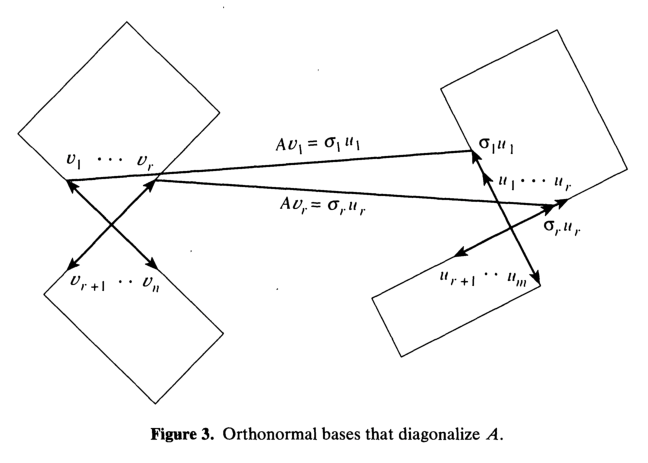
\includegraphics[width=92mm]{strang_fig3}

\vspace{-3mm}
For $V = [\vecnot{v}_1,\ldots,\vecnot{v}_n]
$ and $U = [\vecnot{u}_1,\ldots,\vecnot{u}_m]$, $A V = U \Sigma$ where $\Sigma \in \RealNumbers^{m \times n}$ has diagonal $\sigma_1,\ldots,\sigma_r$.  Thus, $A = U \Sigma V^H$.


\let\thefootnote\relax\footnotetext{\hspace*{-4mm} {\tiny Figure from ``The Fundamental Theorem of Linear Algebra'' by Gilbert Strang, The American Mathematical Monthly, Nov. 1993 }}

\end{frame}




\begin{frame}{6.5: The Four Fundamental Subspaces: Pseudo-Inverse}

\hspace*{-4mm}
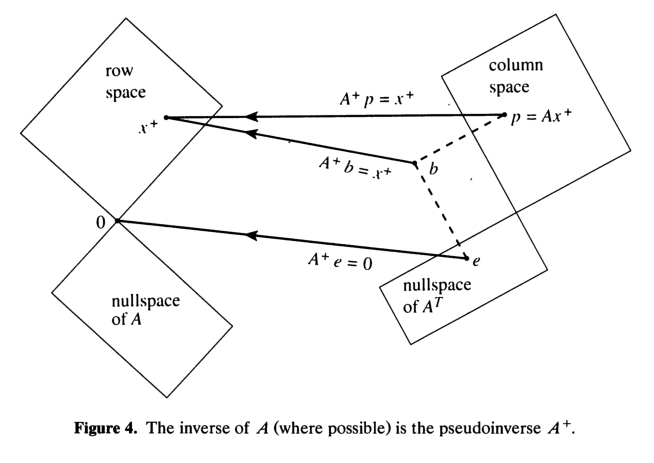
\includegraphics[width=114mm]{strang_fig4}

\let\thefootnote\relax\footnotetext{\hspace*{-4mm} {\tiny Figure from ``The Fundamental Theorem of Linear Algebra'' by Gilbert Strang, The American Mathematical Monthly, Nov. 1993 }}

\end{frame}

\begin{frame}{9.2: Singular Value Decomposition Example}

\visible<1->{%
Consider the matrix \vspace{-2mm}
\[ A = \left[ \begin{array}{cc}
1 & 1 \\
5 & -1 \\
-1 & 5 
\end{array} \right]. \]}

\visible<2->{%
An eigenvalue decomposition of $A^H A$ is given by
\[ \!\!\!\!\!\!\!\!\!\!\!\! A^H A \!=\! \left[ \begin{array}{cc}
27 & -9 \\
-9 & 27
\end{array} \right]
\!=\! V \Lambda V^H
\!=\! \left( \frac{1}{\sqrt{2}}\left[ \begin{array}{cc}
-1 & 1 \\
1 & 1 
\end{array} \right] \right)
\left[ \begin{array}{cc}
36 & 0 \\
0 & 18
\end{array} \right]
\left( \frac{1}{\sqrt{2}} \left[ \begin{array}{cc}
-1 & 1 \\
1 & 1 
\end{array} \right] \right)
\]}

\visible<3->{%
This implies $\Sigma_1 = \Lambda^{1/2}$ and $V_1 = V$.
Thus, we find $U_1 = A V_1 \Sigma_1^{-1}$ with \vspace{-1mm}
\[ U_1 = \left[ \begin{array}{cc}
1 & 1 \\
5 & -1 \\
-1 & 5 
\end{array} \right]
\left( \frac{1}{\sqrt{2}} \left[ \begin{array}{cc}
-1 & 1 \\
1 & 1
\end{array} \right] \right)
\left[ \begin{array}{cc}
\frac{1}{\sqrt{36}} & 0 \\
0 & \frac{1}{\sqrt{18}}
\end{array} \right]
= \left[ \begin{array}{cc}
0 & \frac{1}{3} \\
\frac{1}{\sqrt{2}} & \frac{2}{3}  \\
-\frac{1}{\sqrt{2}} & \frac{2}{3} 
\end{array} \right] \]}

\vspace{-1.5mm}

\visible<4->{%
Putting this all together, we have the compressed SVD \vspace{-1mm}
\[ A = U_1 \Sigma_1 V_1^H 
= \left[ \begin{array}{cc}
0 & \frac{1}{3} \\
\frac{1}{\sqrt{2}} & \frac{2}{3}  \\
-\frac{1}{\sqrt{2}} & \frac{2}{3} 
\end{array} \right]
\left[ \begin{array}{cc}
\sqrt{36} & 0 \\
0 & \sqrt{18}
\end{array} \right]
\left( \frac{1}{\sqrt{2}} \left[ \begin{array}{cc}
-1 & 1 \\
1 & 1 
\end{array} \right] \right). \]}

\end{frame}

\begin{frame}{Moore--Penrose Pseudo Inverse}

For a matrix $A \in \ComplexNumbers^{m\times n}$, the matrix $A^+ \in \ComplexNumbers^{n\times m}$ is the pseudo-inverse iff:
\begin{enumerate}
\item $A A^+ A = A$ (implies $A A^+$ is idempotent)
\item $A^+ A A^+ = A^+$ (implies $A^+ A$ is idempotent)
\item $(A A^+)^H = A A^+$ (implies $A A^+$ is Hermitian)
\item $(A^+ A)^H = A^+ A$ (implies $A^+ A$ is Hermitian)
\end{enumerate}

\begin{lemma}
From the compact SVD $A = U_1 \Sigma_1 V_1^H$, one finds that $A^+ = V_1
\Sigma_1^{-1} U_1^H$.
\end{lemma}

\begin{proof}<2->
\begin{enumerate}
\item $A A^+ A = U_1 {\color{blue}(\Sigma_1 V_1^H  V_1
\Sigma_1^{-1} U_1^H  U_1)} \Sigma_1 V_1^H = A $
\item $A^+ A A^+ =  V_1
{\color{blue}(\Sigma_1^{-1} U_1^H U_1 \Sigma_1 V_1^H  V_1)}
\Sigma_1^{-1} U_1^H  = A^+$
\item $(A A^+)^H = \big(U_1 {\color{blue}(\Sigma_1 V_1^H V_1
\Sigma_1^{-1})} U_1^H \big)^H  = {U_1 U_1^H} = A A^+$
\item $(A^+ A)^H = \big(V_1 {\color{blue}(\Sigma_1^{-1} U_1^H U_1
\Sigma_1)} V_1^H \big)^H  = {V_1 V_1^H} = A^+ A$ \qedhere
\end{enumerate}
\end{proof}

\visible<2->{Thus, $A A^+$ and $A^+ A$ are projection matrices onto $\mathcal{R}(A)$ and $\mathcal{R}(A^H)$.}

\end{frame}

\begin{frame} \frametitle{Approximation Property of the SVD}

\begin{definition}
Let $A \in \mathbb{C}^{m\times n}$ have SVD $A=U \Sigma V^H$ where $\vecnot{u}_1,\ldots,\vecnot{u}_m$ and $\vecnot{v}_1,\ldots,\vecnot{v}_n$ are the columns of $U$ and $V$.
Then, the \textcolor{blue}{$k$-truncated SVD expansion of $A$} is \vspace{-2mm}
\[ \mathcal{T}_k (A) \triangleq \sum_{i=1}^k \sigma_i \; \vecnot{u}_i \, \vecnot{v}_i^H \]
\end{definition}

\vspace{2mm}

\begin{theorem}
In terms of the Frobenius norm $\| A \|_F^2 \triangleq \sum_{ij} |a_{ij}|^2$, the best rank-$k$ approximation of $A \in \mathbb{C}^{m\times n}$ is given by the $k$-truncated SVD expansion: \vspace{-2mm}
\[ \min_{B \in \mathbb{C}^{m\times n}: \, \text{rank}(B)=k} \| A - B \|_F  = \| A - \mathcal{T}_k (A) \|_F \]
\end{theorem}

\vspace{2mm}

The Frobenius norm is induced by inner product $\langle A | B \rangle \triangleq \text{Tr} (B^H A)$ on $\mathbb{C}^{m \times n}$  
\end{frame}

\begin{frame} \frametitle{Principal Component Analysis (PCA)}

\textbf{Problem:} For a given set of $N$ data points $\vecnot x_{1},\vecnot x_{2},\ldots,\vecnot x_{N}\in\mathbb{R}^{n}$, what $p$-dimensional affine subspace $W\subset\mathbb{R}^{n}$ minimizes the approximation error \vspace{-1.5mm}
\[
\sum_{i=1}^{N}\|\vecnot x_{i}-P_{W}(\vecnot x_{i})\|^{2}.
\]

\vspace{-1.5mm}

\textbf{Solution:} Using $\vecnot w_{0}=\frac{1}{N}\sum_{i=1}^{N}\vecnot x_{i}$, we define the mean-corrected data matrix \vspace{-1.5mm}
\[ A=[\vecnot x_{1}-\vecnot w_{0},\ldots,\vecnot x_{N}-\vecnot w_{0}]. \]

\vspace{-1mm}

Then, the problem can solved using the SVD $A=U\Sigma V^{T}$ .
In particular, one can define $U_{p}\triangleq[\vecnot u_{1},\ldots,\vecnot u_{p}]$ and choose $W = \textrm{span}(U_p) + \vecnot{w}_0$ so that \vspace{-1.5mm}
\[ P_{W}(\vecnot x)=U_{p}U_{p}^{T}(\vecnot x-\vecnot w_{0})+\vecnot w_{0} . \]

\vspace{-1mm}

For dimension reduction, one stores $\vecnot y_{i}=U_{p}^{T}\vecnot x_{i}\in\mathbb{R}^{p}$ instead of $\vecnot x_{i}\in\mathbb{R}^{n}$.

\vspace{4mm}

Note: This solution essentially replaces $A$ by the $p$-truncated SVD $\mathcal{T}_p (A)$

%\vspace{2mm}
%
% Recall that an \emph{affine subspace} $W=\text{span}\{\vecnot w_{1},\ldots,\vecnot w_{p}\}+\vecnot w_{0}$ is defined by linearly independent vectors $\vecnot w_{0},\ldots,\vecnot w_{p}$ where adding $\vecnot w_{0}$ has the effect of translating the subspace $\text{span}\{\vecnot w_{1},\ldots,\vecnot w_{p}\}.$ For such an affine subspace, we define $B\in\mathbb{R}^{n\times p}$ by $B=[\vecnot w_{1},\ldots,\vecnot w_{p}]$ and the projection onto $W$ is defined by $P_{W}(\vecnot x)=B(B^{T}B)^{-1}B^{T}(\vecnot x-\vecnot w_{0})+\vecnot w_{0}$.
 


\end{frame}

\begin{frame} \frametitle{Next Steps}

\begin{itemize}
\setlength\itemsep{5mm}
\item To continue studying after this video -- \vspace{2mm}

\begin{itemize}
 \setlength\itemsep{3mm}
 
 \item Try the required reading from website: \\[1mm] \hspace{5mm} The Fundamental Theorem of Linear Algebra by Gilbert Strang
 
 \item Or the recommended reading:  Course Notes EF 6.5 - 6.6.1, 9.1 - 9.3

 \item Also, look at the problems in Assignments 7 and 8
\end{itemize}
\end{itemize}

\note{
	\vspace{8mm}
	\begin{enumerate}
		\setlength\itemsep{3mm}
		\color{red}
		\item Here are some options to continue learning this material. (read) \\ [2mm]  That's it for today.  So, I'll see you next time.
	\end{enumerate}
}

\end{frame}

\end{document}



\backupbegin

%\begin{frame}
%\frametitle{Backup Slides}
%\begin{itemize}
%\item Slide numbers not included in denominator!
%\end{itemize}
%\end{frame}

%\begin{frame}[allowframebreaks]
%\frametitle{References}
%\bibliographystyle{alpha}
%\footnotesize
%\bibliography{IEEEabrv,WCLabrv,WCLbib,WCLnewbib}
%\end{frame}

\backupend

\end{document}
